\chapter{Implementing a multi-architecture posit library}


\section{Overview of existing posit libraries}

In this chapter we will focus on presenting and analyzing posit libraries, including the one created and maintained by us. We will consider the \texttt{C++} based libraries.
Having software support for a new type is of utmost importance. A software library supporting posits should have the following properties:
\begin{enumerate}
    \item Can hot-swap the binary32 \textit{float} type without changing much code
    \item Supports a wide range of posit configurations, typically defined at compile time
    \item Avoids to implement posit operations directly using a $1:1$ hardware correspondence in software 
\end{enumerate}

Property 1) is typically obtained by having a posit type that overloads most of the basic arithmetic operators (e.g. +,-,*,/ and their variations). Furthermore, machine learning and linear algebra applications make extensive use of numerical \textit{traits} to calibrate the algorithms. Therefore, a good posit library should also implement them to fulfil property 1). 

Property 2) can be achieved by templetization of the code. In particular, we should have, at minimum, $2$ template parameters: one for the number of bits $nbits$ and one for the number of exponent bits $esbits$. We will see  in the following sections that we can achieve more degrees of freedom with more templates parameter.

Property 3) is strictly related to the computing performance of the library. In this phase, we pretend not to have any hardware support for the library. Therefore, software emulation of posits occurs. This can be done either by exactly reproducing what a posit-enabled hardware would perform for the various operations or relying on a back-end format for computations. Such a format should have complete hardware support to handle computations efficiently. Property 3) can also be fulfilled with pre-computation of posit operations, thus creating software look-up tables that can be addressed to obtain result of operations without actually computing them.


\subsection{SoftPosit}

SoftPosit \cite{softposit} is one of the first open-source posit libraries appeared. The core is \textit{C} based, but the library offers interfaces for C++, Python and Julia. 

While the core C library obviously does not offer operator overloading, the included C++ API interface offers such feature. However, there is no support for numerical traits inside the C++ interface. Therefore the property 1) we expressed before is not completely satisfied by this library.

SoftPosit offers the following posit configurations:
\begin{itemize}
    \item \posit{32}{2}
    \item \posit{16}{1}
    \item \posit{8}{0}
\end{itemize}

\lstinputlisting[caption={Example of use of SoftPosit with a \posit{8}{0}},label={lst:softPosit8}]{snippets/softposit8example.c}

The posit type is represented by a C \texttt{struct} called  \texttt{posit<bits>\_t}, where \texttt{<bits>} is the number of posit bits. Posit values are stored as signed integers. The size of the integer depends on the size of the posit considered:

\begin{itemize}
    \item \posit{32}{2}: \texttt{posit32\_t} stored in a \texttt{int32\_t}
    \item \posit{16}{1}: \texttt{posit16\_t} stored in a \texttt{int16\_t}
    \item \posit{8}{0} : \texttt{posit8\_t}  stored in a \texttt{int8\_t}
\end{itemize}

These configurations are statically typed inside the library so there is no flexible way to express a desired configuration for the posit at compile time (except for deeply modifying the library). Therefore, property 2) does not hold in this case.

Looking at the internals of SoftPosit we can see that each operation between posit is represented by a function in the format \texttt{p<bits>\_<op>}, where \texttt{<bits>} is the number of posit bits and \texttt{<op>} is the name of the operation (e.g. 'add').

Listing \ref{lst:softPosit8} and \ref{lst:softPosit16} show an example of the C API used to sum two \posit{8}{0} or two \posit{16}{1}.



\lstinputlisting[caption={Example of use of SoftPosit with a \posit{16}{0}},label={lst:softPosit16}]{snippets/softposit16example.c}


Posit operations are implemented following the hypothetical hardware implementation of a posit processing core; indeed, the evaluation of operations not only involves the decoding of the posit to its fields, but also manipulation of such fields to perform the operations. Due to this choice also the property 3) cannot hold.

\section{The cppPosit core}\label{sec:cppPositCore}

The cppPosit library revolves around the idea of a highly template-ized type that can bet dropped in place of the C++ native \texttt{float} in any application. 

The main class of the library is the \textit{posit} class, as reported in Listing \ref{lst:positClassCore}.  

\lstinputlisting[caption={Posit class core},label={lst:positClassCore}]{snippets/positclass.cpp}

The template meaning is the following:
\begin{itemize}
    \item \texttt{class T}: storage (or holder) type for the posit. Typically aligned to power of 2. For example: \texttt{int8\_t}, \texttt{int16\_t}, \texttt{int32\_t}
    \item \texttt{totalbits}, \texttt{esbits}: respectively, the posit parameters for $nbits$ and $esbits$ as shown in previous sections.
    \item \texttt{FT}: backend type for the posit: can be a fixed-point or a floating-point backend (more on this in the following section).
    \item \texttt{positSpec}: specific class to represent a configuration for posit with \textit{Infinity} or \textit{Not a Real} for the North point of the posit ring.
\end{itemize}

The template also enforces some controls over its arguments. Indeed, the value \texttt{totalbits} needs to be lower or equal than the size of the storage type \texttt{T}. Furthermore, the backend type \texttt{FT} needs to be big enough to contain the dynamic range of the represented posit.


\subsection{Operation levels}

When considering posits, we can classify its operations in 4 different levels:

\begin{itemize}
    \item $\mathcal{L}_1$: level-one operations are implemented with a direct manipulation of the posit bit representation (e.g. all the fast-approximated operations seen in previous chapter lie in this level).
    \item $\mathcal{L}_2$: level-two operations need the decoding of the posit into its fields (sign, regime, exponent and fraction). Typically these operations are used to obtain one of the posit fields to manipulate it (e.g. increasing the regime when doubling a posit with more than 0 exponent bits).
    \item $\mathcal{L}_3$: level-three operations require to decode the posit as in $\mathcal{L}_2$ and build the joint regime-exponent value. This operations are required to transform a posit into a format in the FIR space as seen in Section \ref{sec:fir}. A common use of these operations is indeed the conversion of a posit to another floating point format (e.g. IEEE binary32).
    \item $\mathcal{L}_4$: level-four operations require the transformation of a posit to its backend,to compute operators like $+,*,-,/$ and others.
\end{itemize}

\subsection{One frontend, different backends}

As described in the previous Subsection, one of the template arguments of the posit class is the backend type, used to control the actual implementation of posit operations in $\mathcal{L}_4$.

We have 3 different class of backends implemented in cppPosit:
\begin{itemize}
    \item Integral backend (\texttt{Unpacked}): the posit backend is actually the integer where it is stored and the computations are performed emulating an ideal posit processing unit hardware (this is completely similar to the softposit approach).
    \item Floating point backend (\texttt{BackendFloat}): posit computation in $\mathcal{L}_4$ are not performed on the posit representation. Instead, the posit is transformed to a floating point number (e.g. binary32 or binary64) through the FIR representation and then computation are performed using native hardware support for such formats. At the end, the result is converted back to posit. 
    \item Fixed point backend (\texttt{BackendFixed}): this backend exploits fixed-point arithmetic to perform posit computation. Similar to the floating point backend, posit numbers are converted to fixed-point before computations and are reconstructed from fixed-point result after the operations.
\end{itemize}

A particular note on the \texttt{BackendFixed} backend must be outlined: in the library we identify the fixed point backend with a \texttt{FixedTrait} trait template, that contains the number of bits of the fixed point integer to be used. We enforce that this amount of bits is enough to contain the posit dynamic. 

Given a fixed point $Fx$on $L$ bits, we know that the maximum representable value is $2^{L/2 - 1}$ (rounded upwards considering the additional $L/2$ fractional bits). On the other hand, the maximum posit value is $\text{maxposit} = useed^{(nbits - 2)}$. We then need to impose that $max(Fx) \geq maxposit$: 

\begin{equation}
    2^{\frac{L}{2} - 1} \geq  useed^{(nbits - 2)}
\end{equation}

\begin{equation}
    2^{\frac{L}{2} - 1} \geq 2^{2^{esbits} \cdot (nbits - 2)}
\end{equation}

\begin{equation}
    \frac{L}{2} \geq 2^{esbits} \cdot (nbits - 2) + 1
\end{equation}

\begin{equation}
    L \geq 2^{esbits + 1} \cdot (nbits - 2) + 2
\end{equation}

Table \ref{tab:fixedPointToPositSize} summarizes the requirements for the fixed point backend for different posit configurations.

\begin{table}[]
\centering
\caption{Summary of required Fixed point bits for different posit configurations}
\label{tab:fixedPointToPositSize}
\begin{tabular}{lllll}

bits & esbits & useed & min(L) & Fixed point bits \\ \hline
8    & 0      & 2     & 14     & 16               \\
8    & 1      & 4     & 26     & 32               \\
8    & 2      & 16    & 50     & 64               \\
16   & 0      & 2     & 30     & 32               \\
16   & 1      & 4     & 58     & 64               \\
16   & 2      & 16    & 114    & 128              \\ \hline
\end{tabular}
\end{table}

Listing \ref{lst:positDefinitionCppPosit} shows some examples of posit definitions using different backends. A particular definition is the last one. Indeed, we can use more than the needed bits for the fixed point as a posit backend. Doing so, we can reach the point where the fixed point is big enough to hold accumulation of posit values, thus obtaining an accumulator similar to a \textit{quire}.

Having this possibility means that we can implement \textit{multiply-add} operations where consecutive accumulation of posit-posit multiplication are represented on a fixed point big enough not to introduce any rounding during all the process.  

\lstinputlisting[caption={Different Posit definition inside cppPosit},label={lst:positDefinitionCppPosit}]{snippets/positDefinitions.cpp}



\subsection{Fast operations with 0 exponent bits}

As we described in previous Section the cppPosit library has a class of operations in $\mathcal{L}_0$ that can be carried out with bit manipulations of the posit bit representation. We already discussed the accuracy impact of these operations in Section \ref{subsec:fastArithOps}. In \cite{coco_et_al_jrtip_2020, coco2020sensors} we also evaluated the impact on the processing time of such operations, in particular the activation functions.

\begin{figure}
    \centering
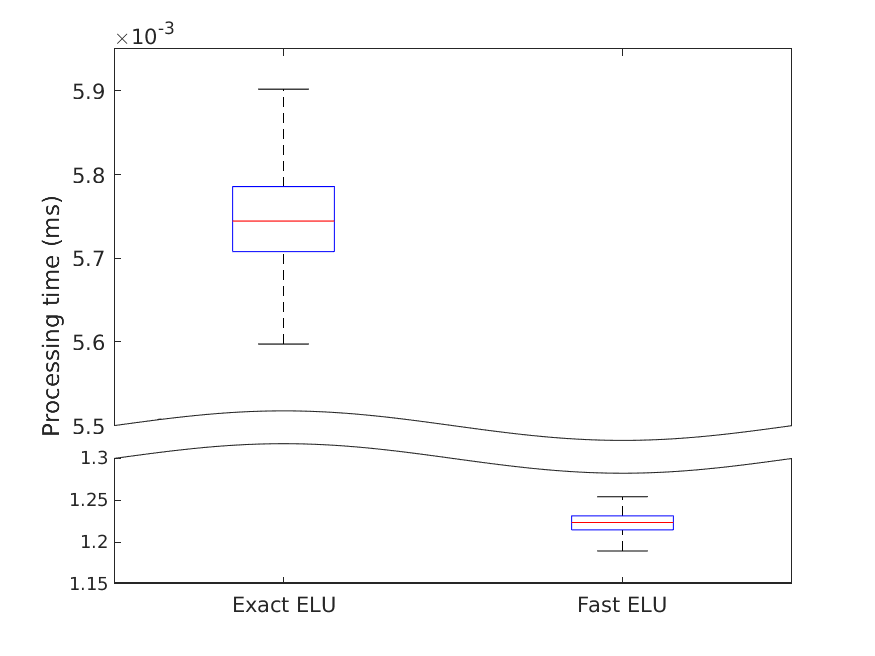
\includegraphics[width=\linewidth]{img/eluTimeComparison.png}
    \caption{Time comparison on the execution of the ELU activation function on the entire \posit{8}{0} domain}
    \label{fig:posit80EluTimeComparison}
\end{figure}

\begin{figure}
    \centering
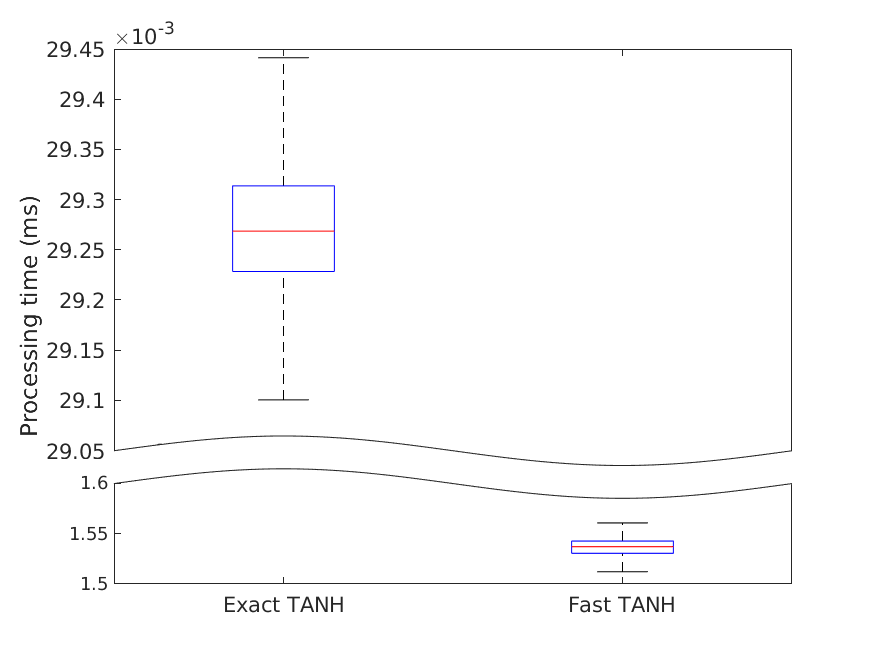
\includegraphics[width=\linewidth]{img/tanhTimeComparison.png}
    \caption{Time comparison on the execution of the TANH activation function on the entire \posit{8}{0} domain}
    \label{fig:posit80ETanhTimeComparison}
\end{figure}

Figures \ref{fig:posit80EluTimeComparison} and \ref{fig:posit80ETanhTimeComparison} show the processing time of the ELU and TANH activation functions evaluated on the entire \posit{8}{0} domain (256 samples). The evaluation was carried out on a 7-th generation \texttt{Intel i7-7560U} processor, running Ubuntu Linux \texttt{18.04}, equipped with \texttt{GCC 8.3}. As we can see from the two plots it is clear how the approximated version outperforms the exact version both in mean value and in variance, being more reliable in the variation of time elapsed for the computation. This stems from the fact that the fast version is evaluated entirely on the ALU, that is traditionally a fixed-latency unit in most of the general purpose processors.

\section{Posit tabulation and logarithmic tabulation}

In the absence of proper hardware support of a Posit Processing Unit (PPU) there still is the need for speeding up the computation. An interesting mean to cope with this problem is the pre-computation of some useful Posit operators in look-up tables. These LUTs become useful when the number of bits is low (e.g. $nbits < 12$).
The core idea is to generate tables for the most important arithmetic operations (addition/subtraction and multiplication/division) for all combination of a given Posit configuration $nbits,esbits$.
Moreover, some interesting functions can be tabulated, in order to speedup their computation, like \textit{logarithm} or \textit{exponentiation}.
Given a $nbits$ bit Posit, with a naive approach, a table will be \[ T \in P^{R \times C} \] where: \[ R=C=2^{nbits}   \]
Depending on the underlying storage type \texttt{T}, each table entry will occupy \texttt{b=sizeof(T)} bits. Typically there will be between $N=8$ and $N=10$ tables for a Posit configuration. This means that the overall space occupation will be \[ S=N \cdot (R \cdot C) \cdot b \]
Table \ref{tab:table_occup} shows different per-table occupation of different Posits configurations. As reported,only Posits with $8$ and $10$ bits have reasonable occupation, considering current generation of CPUs. In fact we can obtain a considerable speedup when one or more tables can be entirely contained inside the cache.

\begin{table}[H]
\centering
\caption{Table occupation for various configurations}
\label{tab:table_occup}
\begin{tabular}{ccc}
\hline \textbf{Total bits (X)}
           & \textbf{Storage type bits (b)}   
           & \textbf{Per-table occupation}
\\ \hline
 \textbf{8} & $8$ & $64$ \textit{KB}\\ \hline
 \textbf{10} & $16$ & $2$ \textit{MB} \\ \hline
 \textbf{12}& $16$ & $32$ \textit{MB} \\ \hline
 \textbf{14}& $16$ & $512$ \textit{MB}\\ \hline
  \textbf{16} & $16$ & $8$ \textit{GB}\\ \hline
\end{tabular}
\end{table}


In order to reduce both LUT size and their number we can exploit some arithmetic properties:
\begin{itemize}
    \item Addition and subtraction are respectively symmetric and anti-symmetric. The two tables can be merged into one and only one half of it is required (above or below the main diagonal).
    \item Multiplication and division can be simplified through logarithm properties. Given $p=x\cdot y$, we can apply $log$ operator on both sides (see \cite{arnold2003interval}), thus obtaining $\log(p) = \log(x\cdot y)$. From logarithm properties this results in \[\log(p) = \log(x)+\log(y)\] Finally, going back with exponentiation we get: \[ p = e^{\log(x)+\log(y)} \] Since tabulation of single operators scales linearly with the Posit size, it is feasible only to store $\exp,\log$ instead of multiplication and division, thus exploiting addition/subtraction LUT for the computation. 
    \item We can compact multiplication tables even more by exploiting the fast inversion (L1) shown in Section \ref{subsec:fastArithOps}. Suppose to have two Posit numbers $x,y$ and their reciprocates, if we want to provide every multiplication or division combination we would build a LUT like in Table \ref{tab:tab_mul_full}. This table would result in 16 entries for only 4 numbers, hence not manageably growing with Posit size. If we apply the L1 inversion and symmetry of negative values, we only need to store the operations for $x\cdot y$ and $x/y$, thus resulting in a LUT size of only 2 elements for the same amount of numbers, as shown in Table \ref{tab:tab_mul_color}.
\end{itemize}

\begin{table}[]
\centering
\caption{All the possible combinations for multiplying and dividing two Posit numbers.}
\label{tab:tab_mul_full}
\begin{tabular}{ccccc}
\hline
\textbf{}     & \textbf{1/x} & \textbf{x} & \textbf{-1/x} & \textbf{-x} \\ \hline
\textbf{1/y}  & 1/xy         & x/y        & -1/xy         & -x/y        \\ \hline
\textbf{y}    & y/x          & xy         & -y/x          & -xy         \\ \hline
\textbf{-1/y} & -1/xy        & -x/y       & 1/xy          & -x/y        \\ \hline
\textbf{-y}   & -y/x         & -xy        & -y/x          & xy          \\ \hline
\end{tabular}
\end{table}

\begin{table}[]
\centering
\caption{All the possible combinations for multiplying and dividing two Posit numbers: all the cells in \textcolor{blue}{blue} correspond to the same LUT entry and the remaining ones correspond to another LUT entry.} \
\label{tab:tab_mul_color}
\begin{tabular}{ccccc}
\hline
\textbf{}     & \textbf{1/x} & \textbf{x} & \textbf{-1/x} & \textbf{-x} \\ \hline
\textbf{1/y}  & \textcolor{blue}{1/xy}         & x/y        & \textcolor{blue}{-1/xy}         & -x/y        \\ \hline
\textbf{y}    & y/x          & \textcolor{blue}{xy}         & -y/x          & \textcolor{blue}{-xy}         \\ \hline
\textbf{-1/y} & \textcolor{blue}{-1/xy}        & -x/y       & \textcolor{blue}{1/xy }         & -x/y        \\ \hline
\textbf{-y}   & -y/x         &\textcolor{blue}{ -xy}        & -y/x          & \textcolor{blue}{xy}          \\ \hline
\end{tabular}
\end{table}

\section{cppPosit in high performance computing environments}
\subsection{ARM Scalable Vector Extension (SVE)}

The ARM Scalable Vector Extension (SVE, \cite{svewhitepaper}) is a vector extension for the ARM AArch64 architecture supported by the ARMv8 instruction set. The main difference between SVE and other single-instruction multiple-data (SIMD) engines (Intel AVX/SSE or ARM NEON) is that it does not specify any width for vector registers, but it provides some constraints for it. The vector register widths must be multiple of $128$ up to $2048$ bits. This approach, called Vector Length Agnostic (VLA), allows us to implement only one vectorized version of our operations, exploiting both auto-vectorization and ARM ACLE (ARM C Language Extensions), without the need to target specific hardware platforms.

\begin{figure}
	\centering    
    \begin{bytefield}[bitwidth=1.5em]{16}
      \colorbitbox{lightcyan}{16}{\scriptsize{Z0 (0..L)}}&\\\\
        \wordbox[]{1}{$\vdots$}\\\\
        \colorbitbox{lightcyan}{16}{\scriptsize{Z31 (0..L)}}&
       
    \end{bytefield}
    \caption{ARM SVE Z Data registers: 32 vector length agnostic register where $L=128\cdot k, k \in [1,16]$}
	\label{fig:zregs}
\end{figure}

\begin{figure}
	\centering    
    \begin{bytefield}[bitwidth=1.5em]{16}
      \colorbitbox{lightgreen}{16}{\scriptsize{P0 (0..P)}}&\\\\
        \wordbox[]{1}{$\vdots$}\\\\
        \colorbitbox{lightgreen}{16}{\scriptsize{P15 (0..P)}}&
       
    \end{bytefield}
    \caption{ARM SVE P predicate registers: 16 vector length agnostic register where $P = Z/8$}
	\label{fig:pregs}
\end{figure}


SVE architecture introduces new kind of registers:
\begin{itemize}
    \item \textit{Z registers}: 32 registers with configurable width, from $128$ to $2048$ bit, as said above. These registers are meant to be data registers. SVE allows to interpret data in Z registers as $8$ bits (bytes), $16$ bits (half-words), $32$ bits (words) and $64$ bits (double-words). For instance, referring to posits, a $2048$ bit Z register can hold up to 256 posit$\left <8,X\right>$ (in any exponent configuration).
    \item \textit{P registers}: 15 predicate registers, with one bit to control each byte in a Z register (a $2048$ bit Z register will be controlled by $256$ bit P register). Each bit in the P register is interpreted as a boolean. A predicate lane, made by $1$ to $8$ predicate bits indicates whether the correspondent lane (when using a Z register) is active or not, depending on the least significant bit.
\end{itemize}


\subsection{RISCV Vector Extension}

The RISC-V \cite{riscvisa} architecture is a modular, open-source and royalty-free instruction set architecture (ISA) and comprises both 32 and 64-bit flavours. The overall ISA is composed of smaller sub-ISAs among which there are the base subsets. These subsets are referred as \textit{base integer instruction sets} and identified by the letter \texttt{I}. Besides, a RISC-V based architecture can present some other extensions; some of them are referred to as \textit{frozen}. This means that their encoding and behaviour has been ratified and will not change during the current draft of the architecture. These extensions include integer multiplication/division operations (\texttt{M}), single (\texttt{F}), double (\texttt{D}) precision floating point operations (following the IEEE 754 Float standard) and atomic instructions (\texttt{A}).

A very interesting and under development extension is the vector one (\texttt{V}). This extension aims to provide single-instruction multiple-data (SIMD) capabilities to the RISC-V architecture. By design, this extension can seamlessly exploit either the CPU registers or a special vector co-processor for hardware acceleration. Any RISC-V based architecture implementing this extension will define some parameters:
\begin{itemize}
    \item Number of vector registers (standard is $32$)
    \item $vlen$: size (in bits) of the vector registers (e.g. $256$)
    \item $elen$: maximum supported size for a single element (e.g. $64$ for a 64-bit integer or double)
\end{itemize}

The idea behind the vector extension is the same of the ARM scalable vector extension (SVE) architecture \cite{armintr}; there is not a predetermined vector length (as happens in the Intel SIMD extensions) but a special instruction \texttt{vsetvl}. This instruction takes as input a requested vector length $vreql$ and returns the granted vector length $vgrant$ as in next expression:
\begin{equation*} %\label{eqn:vsetvl}
    vgrant = \min\left(vlen,vreql\right)
\end{equation*}

This design allows porting an application between RISC-V architectures, without re-writing a single line of code and, in case of furtherly compatible architectures, without recompilation. Moreover, this will help us later when simulating the same program with different vector configurations.

\subsection{cppPosit vector implementation}

In this section, we introduce the vectorized extension of the cppPosit library, aimed to provide the vector version of the posit operations. Firstly, we need to take into account the differences between different operational levels. L1 and L2 operations are the easiest one to be vectorized; they only require bit manipulation of unsigned or signed integers plus additional encoding and decoding steps. Instead, L3 and L4 operations need to be brought back at the chosen backend and then, in case of hardware floating-point we can use native SIMD vectorization if any.

In order to provide a more general and abstract interface to posit vectorized operations, the architecture has separate posit vector frontend and a specialized posit vector backend that, in the paper case, implements the vectorized operations using ARM ACLE for SVE.

\begin{figure*}
\centering
\begin{tikzpicture} 
\umlclass[template=PositT,x=-4,y=0]{PositSVEBackend}{}
{+ vFastSigmoid(vector op,vector dst)  : void } 
\umlclass[type=interface,template=PositT,x=0,y=3]{PositVectorizedFrontend}{}
{+ vFastSigmoid(vector op,vector dst) : void} 
\umlimpl{PositSVEBackend}{PositVectorizedFrontend}
\umlclass[template=PositT,x=4,y=0]{PositRVVBackend}{}
{+ vFastSigmoid(vector op,vector dst) : void} 
\umlimpl{PositRVVBackend}{PositVectorizedFrontend}
\end{tikzpicture}

\caption{UML class diagram for the overall implementation of vectorized operations on posits. Both ARM SVE (left) and RISC-V (right) vectorized operations are supported by our cppPosit library}
\label{fig:cppPositvect}
\end{figure*}

When implementing vectorized operations we have a common template to follow: 
\begin{itemize}
    \item Prologue: we need to prepare the data to be fed to the SIMD engine. For posits and L1 operations, this means preparing a vector with the signed integer representing the posits. In the SVE case this means loading into the $Z$ registers the posit holder type content (e.g. \texttt{int16\_t} for posit$\left<16,X\right>$) using the \texttt{svld1(...)} intrinsic. For L3/4 operations we need instead to unpack the posit to the underlying backend (fixed, floating or tabulated) and load the backend type into registers as well, performing full decoding of the posit type.
    \item Body: the body contains all the arithmetic and logic functions needed to apply the considered operation. In the SVE case, this may contain the SVE intrinsics that operate on the $Z$ vector registers that contain the posit data. For instance, when implementing the fastSigmoid function we will use the built-in intrinsics \texttt{svasr\_x(...)} for the first right shift and \texttt{sv\-add\_x(...)} for the sum. The first performs the same right shift on all the vector elements while the second performs the addition of the value $(1\ll nbits-2)$ to all the vector elements.
    \item Epilogue: we need to build back the posit into the result vector from the signed integer we have just manipulated in the function body. For SVE this means invoking the \texttt{svst1(...)} intrinsic on the SVE result pointer obtained in the previous step. For L3/4 operations we need instead to pack the posit up to the frontend, performing a full encoding of the posit type.
\end{itemize}

When vectorizing non-L1 operations that require the posit to be decoded in its components (sign, regime, exponent and fraction) we need to take into account two phases of the prologue. The first and simplest one is the posit conversion to the underlying signed integer holder type, that is the cost of a pointer cast from the posit type to the holder one. This step has practically no cost. The second and hardest one is the vectorization of the posit decoding step since it involves many operations and branches on the bit-string. After this decoding, the function body is the same as applying vectorization to the backend type (native ARM floats in our case).

The same behaviour holds for the epilogue as well.
Predictably, both prologue and epilogue for non-L1 operations will introduce some kind of overhead in function computation, due to the conversion of the posit at the underlying backend. This means that, to see real effectiveness of this vectorized approach we need to test this on large-sale data and SVE vector sizes.



\begin{algorithm}
 \caption{Posit decoding algorithm (simplified): \textit{signBit} is the posit most significant bit, \textit{extraBits} takes into account of underlying holder type that may not be aligned with the posit size (e.g. \posit{10}{x} stored in an $int16\_t$ type), \textit{positHolderMSB} is the holder type most significant bit. The \textit{findLeftMostSet} function is used to find the index of the first set bit starting from the most significant bit. It is commonly known as \textit{count leading zeroes} (CLZ). The \textit{getBitSetLeft(bitstring,n)} is used to extract \textit{n} bits from \textit{bitstring} starting from the most significant one.}
 \label{alg:positdec}
 \begin{algorithmic}[1]
 \renewcommand{\algorithmicrequire}{\textbf{Input:}}
 \renewcommand{\algorithmicensure}{\textbf{Output:}}
 \Require positRepresentation
 \Ensure sign,regime,exponent,fraction
    \State \textbf{sign} = (positRepresentation \& signBit) != 0
    \State pa = sign ? -positRepresentation : positRepresentation
    \State pars = pa $\ll$ (extraBits+1)
    \State stop = (pars \& positHolderMsb) != 0
    \State index = stop ? findLeftMostSet($\sim$pars) : findLeftMostSet(pars)
    \State \textbf{regime} = stop ? index - 1 : -index
    \State regimeLength = index + 1
    \State pars = pars $\ll$ regimeLength
    \State \textbf{exponent} = getBitSetLeft(pars,esbits)
    \State \textbf{fraction} = pars $\ll$ esbits \Comment{Fraction in MSBs}
\end{algorithmic} 
\end{algorithm}


\begin{algorithm}
 \caption{Float to posit conversion algorithm (simplified). The \textit{pack} function at line 11 is used to build the posit representing integer using the field built in the algorithm: if the sign is negative, we firstly compute the posit for the positive value than we apply the 2's complement to the posit fields to change sign.}
 \label{alg:positenc}
 \begin{algorithmic}[1]
 \renewcommand{\algorithmicrequire}{\textbf{Input:}}
 \renewcommand{\algorithmicensure}{\textbf{Output:}}
 \Require floatRepresentation
 \Ensure positRepresentation
\State sign = (floatRepresentation \& floatSignBit) != 0
\State fExponent = (floatRepresentation $\ll$ 1) $\gg$ 24
\State normFExponent = fExponent - 127
\State fFraction = (floatRepresentation $\ll$ 9) \Comment{Fraction in MSBs}
\State pRegime = normFExponent/esbits
\State pRegimeBits = pRegime + 1
\State expBits = min(nbits - pRegimeBits - 1,esbits)
\State fracBits = nbits - pRegimeBits - 1 - expBits
\State pExp = normFExponent - pRegime 
\State pFrac = fFraction $\gg$ (nbits - fracbits)
\State positRepresentation = pack(sign,pRegime,pExp,pFrac)
\end{algorithmic} 
\end{algorithm}

\begin{algorithm}
 \caption{ Count Leading Zeros (CLZ) function implemented using bit manipulation only: an example for a 16-bit integer}
 \label{alg:clz}
 \begin{algorithmic}[1]
   \renewcommand{\algorithmicrequire}{\textbf{Input:}}
 \renewcommand{\algorithmicensure}{\textbf{Output:}}
 \Require unsignedInt16
 \Ensure firstSet
  \State firstSet = (bitString $>$ 0xFF) $\ll$ 3; bitstring $\gg$ firstSet
  \State q = (bitString $>$ 0xF) $\ll$ 2; bitstring $\gg$ q
  \State firstSet = firstSet $|$ q
  \State q = (bitString $>$ 0x3) $\ll$ 1; bitstring $\gg$ q
  \State firstSet = firstSet $|$ q
  \State firstSet = firstSet $|$ (bitString $\gg$ 1)
 \end{algorithmic}
\end{algorithm}

%\section{Posit-based linear algebra in vector processors}
%\subsection{Exploiting integer-only arithmetic in L1 operations}
%\subsection{L2-4 operations: general problem formulation}
%\subsection{Two examples: convolution and matrix multiplication}

